

\subsection{3D Axis Configuration}
This section described keys which are used to configure the appearance of three dimensional figures. Some of them apply for twodimensional plots as special case as well, and they will also be discussed in the respective sections of this manual.

\begin{pgfplotskey}{view=\marg{azimuth}\marg{elevation} (initially \{25\}\{30\})}
	Changes both view angles of a 3D axis. The azimuth (first argument) is the horizontal angle which is rotated around the $z$ axis. For a 3D plot, the $z$ axis always points to the top. The elevation (second argument) is the vertical rotation around the (rotated) $x$ axis. Positive elevation values indicate a view from above, negative a view from below. All values are measured in degree.

\pgfplotsexpensiveexample
\begin{codeexample}[]
\begin{tikzpicture}
	\begin{axis}[view={0}{0},
		xlabel=$x$,
		zlabel=$z$,
		title=View along the positive $y$ axis]
		\addplot3[surf] {x};
	\end{axis}
\end{tikzpicture}
\end{codeexample}

\pgfplotsexpensiveexample
\begin{codeexample}[]
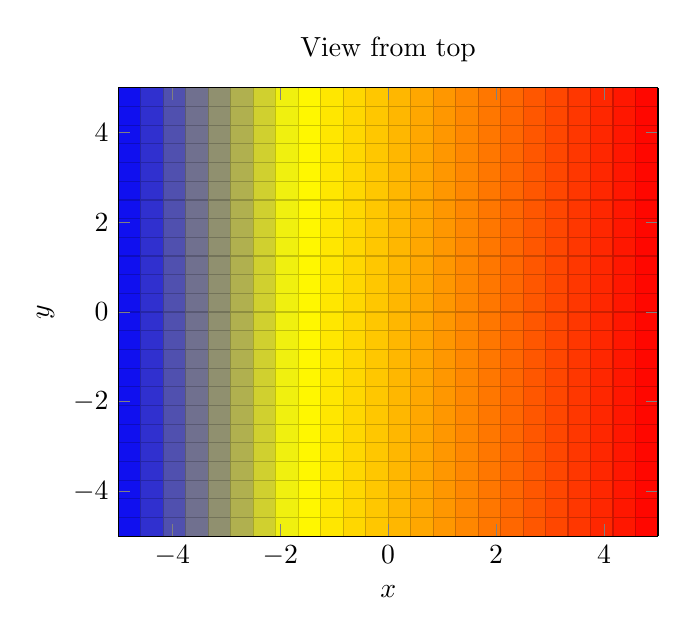
\begin{tikzpicture}
	\begin{axis}[view={0}{90},
		xlabel=$x$,
		ylabel=$y$,
		title=View from top]
		\addplot3[surf] {x};
	\end{axis}
\end{tikzpicture}
\end{codeexample}

\pgfplotsexpensiveexample
\begin{codeexample}[]
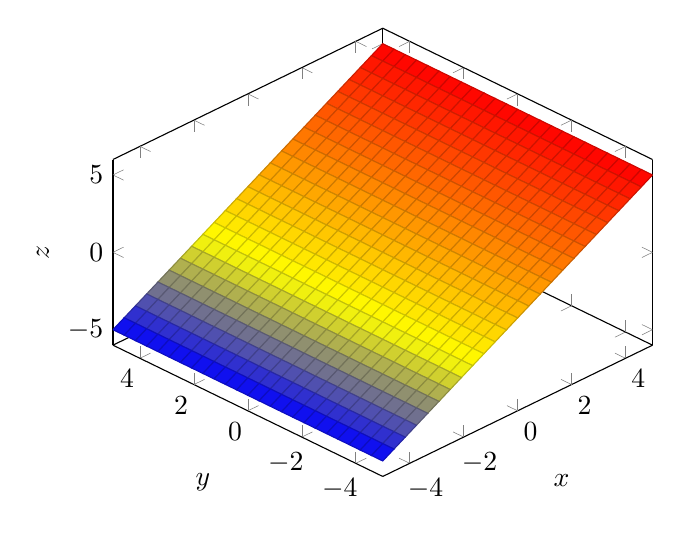
\begin{tikzpicture}
	\begin{axis}[view={-45}{45},
		xlabel=$x$,ylabel=$y$,zlabel=$z$]
		\addplot3[surf] {x};
	\end{axis}
\end{tikzpicture}
\end{codeexample}
\end{pgfplotskey}

\begin{pgfplotskeylist}{view/az=\marg{azimuth},view/h=\marg{azimuth} (initially 25)}
	Changes only the azimuth view angle, i.e.\ the horizontal (first) view angle which is rotated around the~$z$ axis.

\pgfplotsexpensiveexample
\begin{codeexample}[]
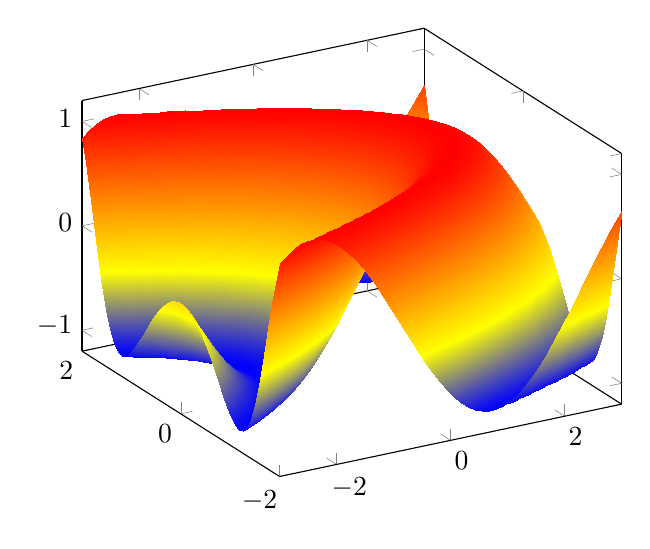
\begin{tikzpicture}
	\begin{axis}[view/h=-30]
	\addplot3[
		surf,
		shader=interp,
		samples=50,
		domain=-3:3,y domain=-2:2] 
		{sin(deg(x+y^2))};
	\end{axis}
\end{tikzpicture}
\end{codeexample}

\pgfplotsexpensiveexample
\begin{codeexample}[]
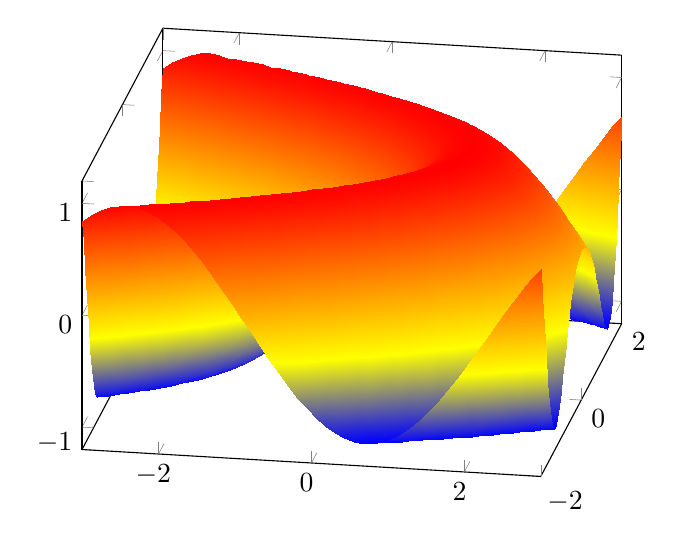
\begin{tikzpicture}
	\begin{axis}[view/h=10]
	\addplot3[
		surf,
		shader=interp,
		samples=50,
		domain=-3:3,y domain=-2:2] 
		{sin(deg(x+y^2))};
	\end{axis}
\end{tikzpicture}
\end{codeexample}

\pgfplotsexpensiveexample
\begin{codeexample}[]
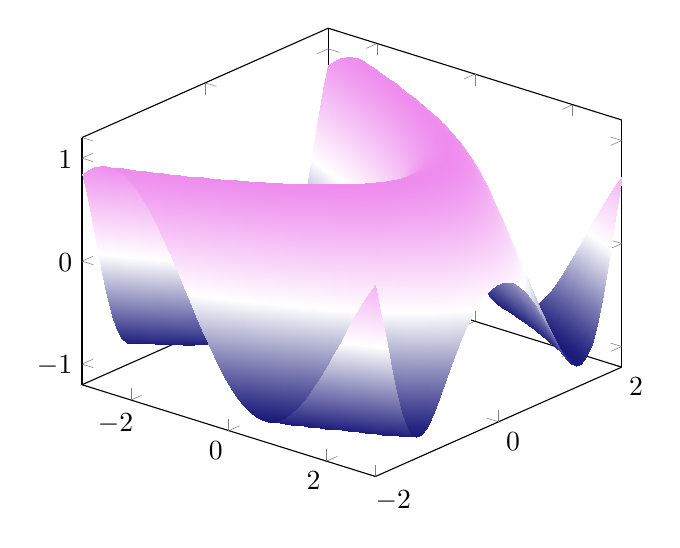
\begin{tikzpicture}
	\begin{axis}[view/h=40,colormap/violet]
	\addplot3[
		surf,
		shader=interp,
		samples=50,
		domain=-3:3,y domain=-2:2] 
		{sin(deg(x+y^2))};
	\end{axis}
\end{tikzpicture}
\end{codeexample}

\pgfplotsexpensiveexample
\begin{codeexample}[]
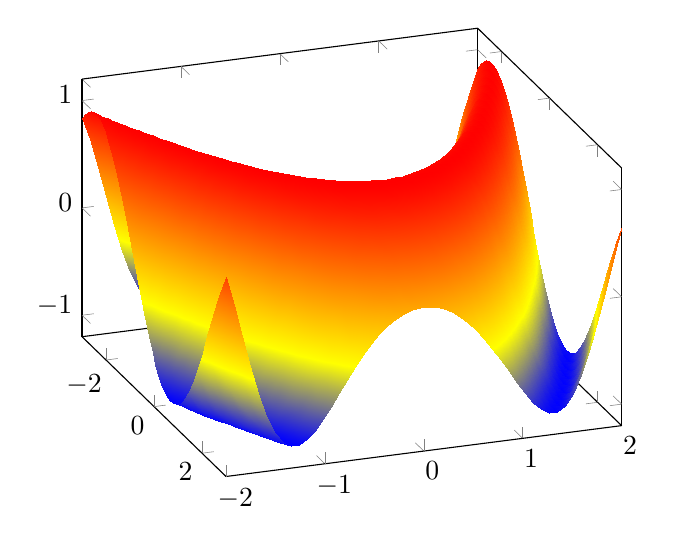
\begin{tikzpicture}
	\begin{axis}[view/h=70]
	\addplot3[
		surf,
		shader=interp,
		samples=50,
		domain=-3:3,y domain=-2:2] 
		{sin(deg(x+y^2))};
	\end{axis}
\end{tikzpicture}
\end{codeexample}
\end{pgfplotskeylist}

\begin{pgfplotskeylist}{view/el=\marg{elevation},view/v=\marg{elevation} (initially 30)}
	Changes only the vertical elevation, i.e.\ the second argument to |view|. Positive values view from above, negative values from below. 
\end{pgfplotskeylist}

\begin{stylekey}{/pgfplots/every 3d description}
	This style is a relatively low level method to change the appearance of \emph{descriptions} for three dimensional axes. Naturally, a three dimensional axis will display axis labels for $x$ and $y$ differently  than a two dimensional axis (for example, the $y$ axis label won't be rotated by 90 degrees). The \declaretext{every 3d description} style installs the necessary display options for three dimensional axis descriptions.

	The initial value is:
\begin{codeexample}[code only]
/pgfplots/every 3d description/.style={
	% Only these description styles can be changed here:
	/pgfplots/every axis x label/.style={at={(ticklabel cs:0.5)},
		anchor=near ticklabel},
	/pgfplots/every axis y label/.style={at={(ticklabel cs:0.5)},
		anchor=near ticklabel},
	/pgfplots/every x tick scale label/.style={
		at={(xticklabel cs:0.85,10pt)},
		anchor=near xticklabel,inner sep=0pt},
	/pgfplots/every y tick scale label/.style={
		at={(yticklabel cs:0.85,10pt)},
		anchor=near yticklabel,inner sep=0pt}
}%
\end{codeexample}

	As the name suggests, |every 3d description| can only be used to set styles for axis labels, tick labels and titles. It has \emph{not} been designed to reset other styles, you will need to change these options either for each axis separately or by means of user defined styles. The reason for this limitation is: other options can (and, in many cases) need to be set before the axis is processed. However, the decision whether we have a two dimensional or a three dimensional axis has to be postponed until the processing is more or less complete -- so only some remaining keys can be set.	
\end{stylekey}

\begin{stylekey}{/pgfplots/every 3d view \marg{h}\marg{v}}
	A style which can be used for fine tuning of the output for specific views.

	This style will be installed right after |every 3d description|, but before other axis description related keys are set (in other words: it has higher precedence than |every 3d description| but less precedence than keys provided to the axis directly).

	One example is preconfigured for |view={0}{90}| (from top):
\begin{codeexample}[code only]
/pgfplots/every 3d view {0}{90}/.style={
	/pgfplots/xlabel near ticks,
	/pgfplots/ylabel near ticks,
	/pgfplots/axis on top=true
}
\end{codeexample}
\end{stylekey}

\begin{pgfplotskeylist}{%
	xticklabel shift=\marg{dimension} (initially 0cm),%
	yticklabel shift=\marg{dimension} (initially 0cm),%
	zticklabel shift=\marg{dimension} (initially 0cm)}
	FIXME
\end{pgfplotskeylist}

\begin{pgfplotsxykey}{\x ticklabel anchor=\mchoice{auto,paraxial,tikz} (initially auto)}
	FIXME
\end{pgfplotsxykey}

\begin{pgfplotskey}{plot box ratio=\marg{x stretch}\marg{y stretch}\marg{z stretch} (initially {1}{1}{1})}
	Allows to customize the aspect ratio between the three different axes in a three dimensional plot.

	The |plot box ratio| is applied before any rotations and stretch--to--fill routines have been invoked. Thus, the initial setting |{1}{1}{1}| makes all axes equally long.

\pgfplotsexpensiveexample
\begin{codeexample}[]
\begin{tikzpicture}
\begin{axis}[
	view/h=60,
	plot box ratio={1}{1}{1},
	colormap={violet}{[1cm] rgb255(0cm)=(25,25,122)
		color(1cm)=(white) rgb255(5cm)=(238,140,238)},
	xlabel=$x$,
	ylabel=$t$,
	zlabel={$p(x,t)$},
	shader=faceted,
	title=Initial \texttt{plot box ratio},
]
	\addplot3[surf,y domain=0.02:3.5,samples=81]
		{1/(2*sqrt(pi*y)) * exp(-x^2/y)};
\end{axis}
\end{tikzpicture}
\end{codeexample}

\pgfplotsexpensiveexample
\begin{codeexample}[]
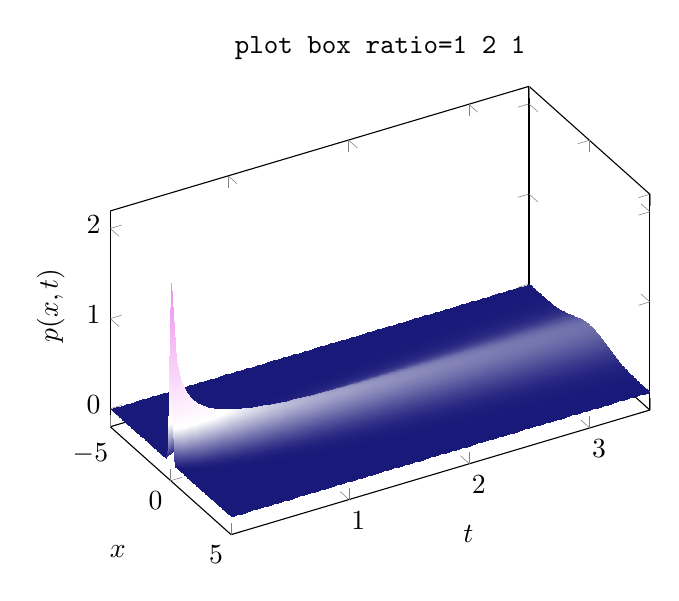
\begin{tikzpicture}
\begin{axis}[
	view/h=60,
	plot box ratio={1}{2}{1},
	colormap={violet}{[1cm] rgb255(0cm)=(25,25,122)
		color(1cm)=(white) rgb255(5cm)=(238,140,238)},
	xlabel=$x$,
	ylabel=$t$,
	zlabel={$p(x,t)$},
	shader=interp,
	title=\texttt{plot box ratio=1 2 1},
]
	\addplot3[surf,y domain=0.02:3.5,samples=81] 
		{1/(2*sqrt(pi*y)) * exp(-x^2/y)};
\end{axis}
\end{tikzpicture}
\end{codeexample}

	This key applies only to three dimensional axes. After the scaling, the axes will be stretched to fill the |width| and |height| for this plot. Thus, the effects of |plot box ratio| might be undone by this stretching for particular views.
\end{pgfplotskey}